% dropbox
\documentclass[12pt,a4paper]{article}

\usepackage{bibtopic}
\usepackage{lec}
%\bibliographystyle{plain}

\usepackage{color}
\usepackage{geometry}

\usepackage{amsfonts}
\usepackage{amsthm}
\usepackage{graphicx}
\usepackage{url}

\usepackage{multicol}
\setlength{\columnsep}{1cm}
\usepackage{lipsum}

% from lanqing
%\usepackage{defs}
\usepackage{amsmath}
\usepackage{bm}


\geometry{left=1in, right=1in, top=1in, bottom=1in}
%\newcommand{\C}{{\cal C}}

%\newcommand{\U}{{\cal U}}

\newcommand{\ff}{{\bf f}}
\newcommand{\hr}{{\hat r}}

%\newcommand{\myskip}[1]{ }
\newcommand{\myskip}[1]{#1}

%\pagestyle{empty}



\begin{document}



\title{XAI-Guided Interventional Retraining for Domain Adaptation}

\date{}

\maketitle


Models trained in one domain usually do not perform well in other domains. For example, models trained on ImageNet have  much lower accuracies on ImageNet V2.  {\em Domain adaptation} is about learning models that generalize well across domains.\\


In this note, I describe a method for domain adaptation that consists of two training phases: (1) regular training, and (2) interventional retraining (IR).
When classifying an input image, the output depends on (1) the object(s) of interest in the image, and (2) the background.  The purpose of IR is to reduce the impact of the background.  It is guided by XAI. So, we call it {\em  XAI-Guided Interventional Retraining (XGIR)}.\\




Let $\{\x_i, y_i\}_{i=1}^N$ be our training data. During regular training, we obtain a feature mapping $h = f_{\theta}(\x)$, which converts the data into $\{h_i, y_i\}_{i=1}^N$. We also obtain a Softmax model $P(y|h, w)$.  XGIR will change only $w$, but not $\theta$. It does so by converting
$\{h_i, y_i\}_{i=1}^N$ into $\{h'_i, y_i\}_{i=1}^N$ and then retrain a softmax model  on the new data.\\


Given  $f_{\theta}(\x)$, $P(y|h, w)$ and  $\{\x_i, y_i\}$, we obtain $h'_i$ as follows:

\bit
\item Run CWOX to get a XAI heatmap $\be_i$ for $y_i$  
    \bit
    \item It could be the heatmap for the class $y_i$ itself  (See Figure \ref{cwox} (b.1))
    
   \item Or, the heatmap for the confusion cluster that contains $y_i$ (See Figure \ref{cwox} (c))
    \eit
\item $\x'_i = \x_i \odot supp(\be_i, \delta_1)$, where $\delta_1$ is a small hyper-parameter, e.g., 0.01.  After this step, some of the background is removed. Some foreground is also removed. Hope it does not matter much.  \\

    $\x'_i$ is the {\bf core} part of $\x_i$ that contains the evidence for the class $y_i$. It is the part the a good model should consider when classifying $\x_i$ into class $y_i$.

\item Let $\r_i  = f_{\theta}(\x'_i) - f_{\theta}(\x^0))$, where  $\x^0$ is the empty image. $\r_i$ is a vector over the units of the feature layer. Ideally, the classifier should relying those units
    with high values $\r_i(u)$.

\item We {\bf intervene} to change feature values $h_i(u)$ for units with low  $\r_i(u)$ via {\bf randomization}:

     \[h'_i(u) = (1 - \lambda_i(u)) h_i(u) + \lambda_i(u) \epsilon_i,\]
     where $\epsilon_i$ is random noise generated from a Gaussian distribution, and

  \[ \lambda_i(u)   = \frac{1}{\delta_2} [\delta_2 - \min\{\delta_2, \r_i(u)\}].\]
     The hyper-parameter $\delta_2$ determines which units are considered to be the core units that capture the information that $y_i$ should rely on.  \\

     In fact, if $\r_i(u) \geq \delta_2$,
     than $h'_i(u) = h_i(u)$.  The feature is not changed as all. If  $\r_i(u) =0$, on the other hand,
      $h'_i(u) =  \epsilon_i$ is a purely random value.  {\bf The model needs to learn not to rely on it}.


\eit


In the project, try the idea on the setup used in the Two-Stage Classification project.

\begin{figure}[t]
\centering

\begin{tabular}{cccccc}
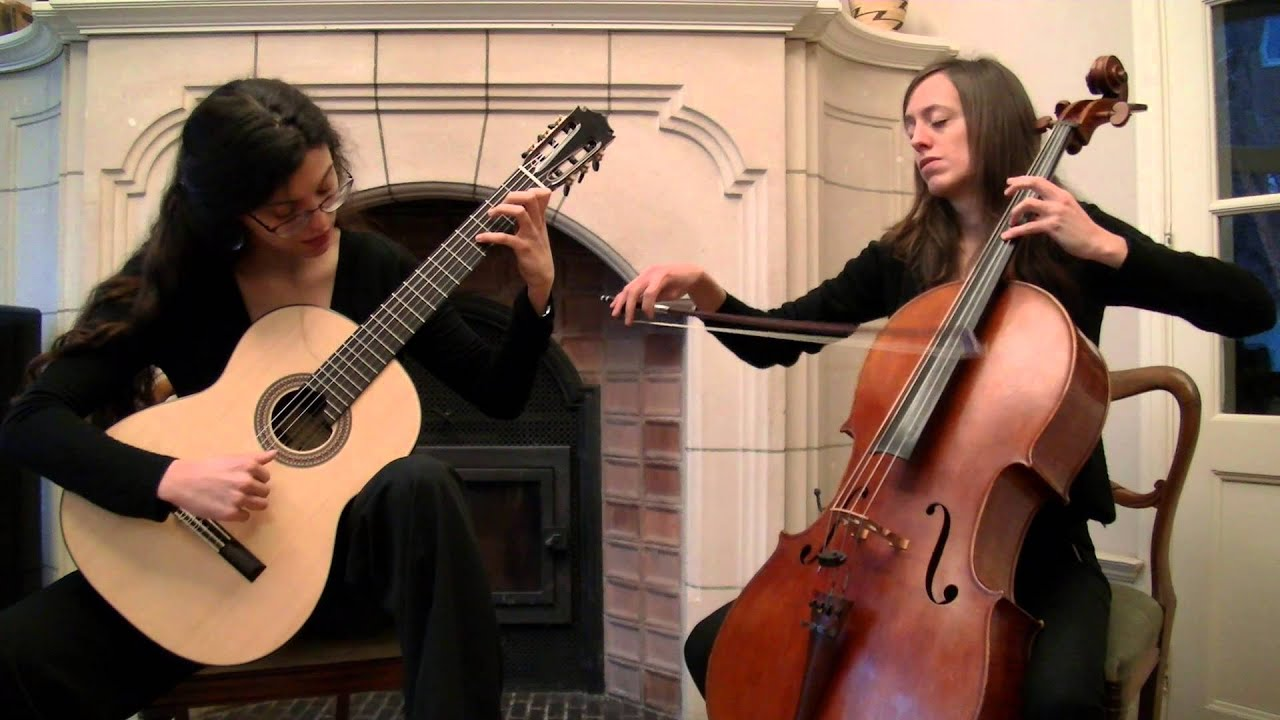
\includegraphics[width=2.8cm, height=2.6cm]{Fig/fig1/guitar-cello.JPG}&
 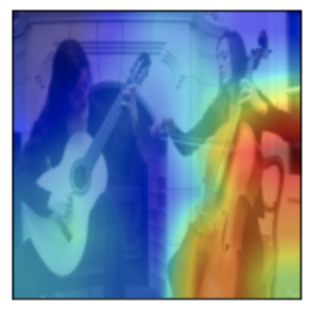
\includegraphics[width=2cm]{Fig/fig1/BPZ/cello.png}&
 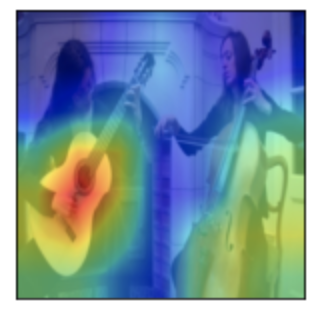
\includegraphics[width=2cm]{Fig/fig1/BPZ/acoustic-guitar.png}&
 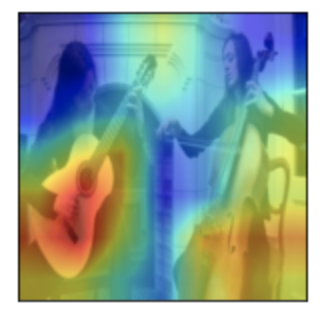
\includegraphics[width=2cm]{Fig/fig1/BPZ/banjo.png}&
 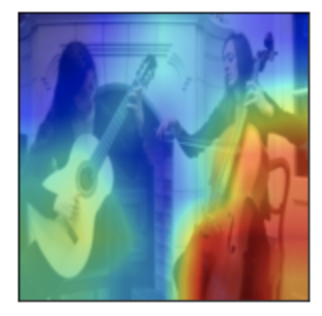
\includegraphics[width=2cm]{Fig/fig1/BPZ/violin.png}&
 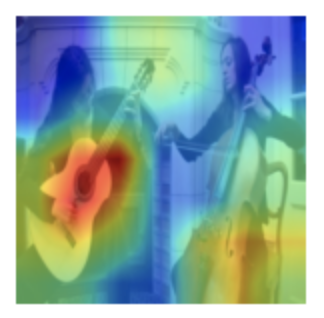
\includegraphics[width=2cm]{Fig/fig1/BPZ/electric-guitar.png}    \\
 {\scriptsize  (a) Input } & {\scriptsize  (b.1) Cello }  & {\scriptsize  (b.2) Acoustic Guitar }  &{\scriptsize  (b.3) Banjo} & {\scriptsize (b.4) Violin} & {\scriptsize  (b.5) Electric Guitar}   \\
\end{tabular}


\begin{tabular}{cccc}
 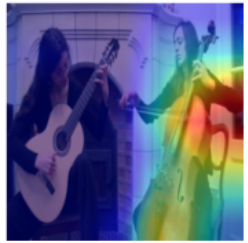
\includegraphics[width=2.5cm]{Fig/fig2/inter1.png}&
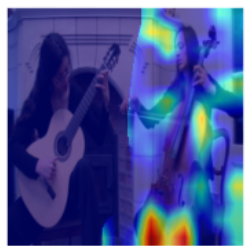
\includegraphics[width=2cm]{Fig/fig2/intra1.png}&
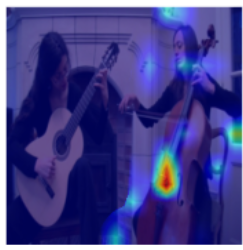
\includegraphics[width=2cm]{Fig/fig2/intra2.png}&
   \\
 {\scriptsize  (c) Cluster 1  }   &  {\scriptsize  (c.1) Cello  }  &{\scriptsize  (c.2) Violin  } & \\
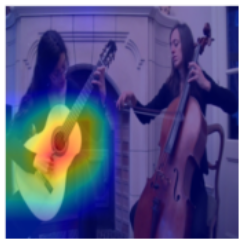
\includegraphics[width=2.5cm]{Fig/fig2/inter2.png}&
 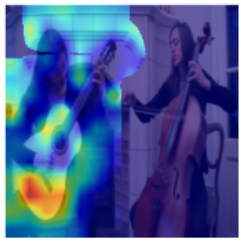
\includegraphics[width=2cm]{Fig/fig2/intra3.png}&
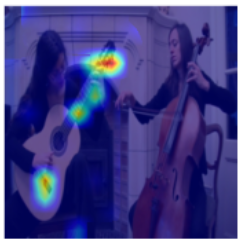
\includegraphics[width=2cm]{Fig/fig2/intra4.png}&
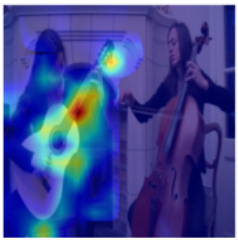
\includegraphics[width=2cm]{Fig/fig2/intra5.png}
   \\
{\scriptsize (d) Cluster 2 } &  {\scriptsize  (d.1) Acoustic Guitar  }   &  {\scriptsize  (d.2) Banjo }  &{\scriptsize  (d.3) Electric Guitar }
\end{tabular}
\caption{\small Individual output explanation (IOX), simple whole-output explanation (SWOX), and contrastive whole-output explanation (CWOX):
(a) Input image with ground-truth label {\tt cello}; (b.1) Grad-CAM heatmap for the top class (IOX); (b.1) - (b.5) Grad-CAM heatmaps for all 5 top classes (SWOX);
(c) - (d) CWOX: Contrastive heatmaps are generated to first contrast the two  confusion clusters (c, d), and then to contrast the classes  in each confusion cluster against  each other (c.1, c.2; d.1, d.2, d.3).
 }
\label{cwox}
\end{figure}



\end{document} 